\documentclass[a4paper,11pt,twoside]{article}

%\usepackage{ngerman}
\usepackage[sort]{natbib}
\renewcommand\bibfont{\small}
\usepackage[pdftex]{graphicx}
\usepackage[pdftex]{color}
\usepackage[
	  bookmarks,
	  bookmarksopenlevel=2,
	  pdfpagelayout=SinglePage,
	  colorlinks=true,
	  pdfstartview=FitV,
	  linkcolor=blue,
	  citecolor=blue,
	  urlcolor=blue]{hyperref}
\usepackage{url}
\usepackage{latexsym}
\usepackage{amsmath,amscd,amsthm}
\usepackage{amssymb}
\usepackage{amsfonts}
\usepackage[latin1]{inputenc}


\bibliographystyle{chicago} 
\citestyle{agsm}


\begin{document}

%\selectlanguage{english} % english,ngerman

\title{Project Plan\\
{\normalsize Master Practicum ``Android OS'', WS 2012/13}}


\author{%
  Zaur Molotnikov, Bibek Shretsha\\%
  \texttt{\url{zaur.molotnikov/bibek.shretsha@in.tum.de}}%
}



\maketitle



\pagebreak


\begin{abstract}
This document is a rough project plan, a part of the Android OS Master Practicum, MSc Informatics program at TUM.
In the document we describe the idea of an upgrade for the AnkiDroid software, 
which lie in the basis of the project as well as try to come up with time estimations on each of the parts.
We shortly discuss, why we think the ideas are challenging and important, together with criteria or goals we put on the 
resulting work. We mention here the desired process model, we are going to take in order to reach the goals.
\end{abstract}

\pagebreak

\tableofcontents

\pagebreak

\section{Introduction}
\label{sec:intro}
AnkiDroid is an Android user interface (UI) for the bigger Anki project. The project contains desktop cross-platform 
application, web-application and services, as well as mobile client or UI. 

The whole goal of the Anki software is enabling the user to learn new information, by memorizing cards. The software,
however is different from many memory-cards applications in some ways. First, it has an algorithm to track, how well
the user is remembering the information, advising on which cards has to be repeated on a particular date.


The cards have usually two sides, and thus represent an entity in the data base with two most-meaningful fields. The
user composes sets of the cards, which are called decks. And then has chance to review the composed decks. The program
allows manipulation with decks, such as: generating new cards from existing ones (for example, through reverting),
sharing decks on the web server, exchanging decks with other Anki users, synchronizing decks (and the usage info) among 
different Anki clients a single user may run.





Potential usages for the learning application with cards could be, \citet{ankinet}:
\begin{enumerate}
  \item learning a language
  \item studying for medical and law exams
  \item memorizing people's names and faces
  \item brushing up on geography
  \item mastering long poems
  \item practicing guitar chords
\end{enumerate}
plus, what we identified is could also be possible:
\begin{enumerate}
  \item learning pronunciation
  \item learning music types 
  \item learning chemistry formulas
  \item teaching children
  \item developing visual memory
\end{enumerate}

However, the full capability of all learning techniques can only be achieved by a powerful enough cards
application, which would support different sorts of content on the cards. For example, to study formulas
(either in chemistry, or mathematics) the graphical content would be much more appropriate, than textual.
To memorize people's names and faces, as the project creator suggest, also photos are essential. Learning
a foreign language put other demands on the application: it has to support pronunciation of complicated words,
(like ``Wiedervereinigung'', German for reuniting, or ``Dostoprimechatelnosti'', Russian for sights), as well 
as different fonts, to show Arabic spelling or hieroglyphs.


Displaying of such content is a must for the application. However, on a modern mobile device, the creation 
of such content could be especially productive, due to high interactivity level with the user. One could imagine
recording voice from the microphone, capturing photos on the camera, or drawing illustrations with the sensor 
screen capabilities.

\begin{figure}[t]
\centering
\label{fig:Graphics}
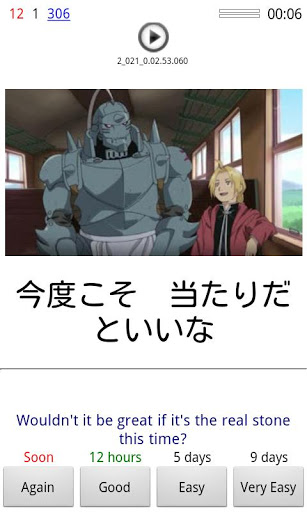
\includegraphics[width=5cm]{Screenshot1}
\caption{AnkiDroid Screenshot : Imported from PC version graphics, is not possible to input in AnkiDroid}
\end{figure}


Unfortunately, such mentioned features are currently missing from the Android implementation of Anki, but 
are required by community, and are constantly asked for \citet{ankigcode}


The existing implementation of AnkiDroid contains only raw textual input. Simply adding a better WYSIWYG editor 
for the text to have styles there, would be a great improvement. However this is not the main target for us.

Often while learning something the user starts from something he/she does not know. This causes a need to search for
knowledge. In a context of the Android application for cards, it would mean many steps process to finish one cards:

\begin{enumerate}
  \item unknown information found (for example, in a browser)
  \item new deck or simply new cards started in Anki
  \item search for the meaning started (browser, photo application, etc.)
  \item needed meaning found
  \item second side of the card filled in back in Anki
\end{enumerate}

The required application switch process decreases user productivity. Moreover, due to the 
nature of Android activities life cycle, it could be, that within such switching, due to the lost
of a current state, the user will need to repeat the work twice (creating cards, after unfinished was discarded, for example).
This motivates adding to the application itself information providing capabilities. Among such capabilities we 
consider the usage of embedded recording and capturing devices, as well as search on the available on the Web resources
for information (for example, Google images sarch, Beolingus dictionary, Wikipedia, etc.)

Summarizing, there is a broad spectrum of opportunities towards improving in a meaningful and requested by community
way the application. Trying to implement some of the mentioned features for the application represents the goal for the project.


\begin{figure}[t]
\centering
\label{fig:Learnproc}
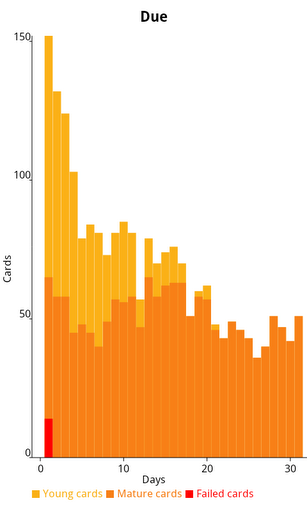
\includegraphics[width=5cm]{Screenshot2}
\caption{AnkiDroid Screenshot : Displaying learning progress}
\end{figure}


It is worth mentioning, that dislike many existing student toy-applications, the modification of AnkiDroid represents a real world project.
The application for the Android under question is not only extremely popular (more than 100.000 downloads), but is also very reliable,
and has clear above average (4.5+) rating. Application represents a client for Android, however it must well integrate with all other
existing clients as well as the web service, provided by Anki project, which enables, for example deck exchange.

Thus development features on top of such application:
\begin{enumerate}
  \item is a challenging task for student level programmers
  \item requires certain level of quality during development
  \item requires maturity of each feature for publishing
  \item allows for real-world project experience
  \item puts consideration on the visual integrity with existing software
  \item introduces need to research on the existing code base, and
  \item brings up the need in considering and validating integration
\end{enumerate}


\begin{figure}[t]
\centering
\label{fig:Downloddeck}
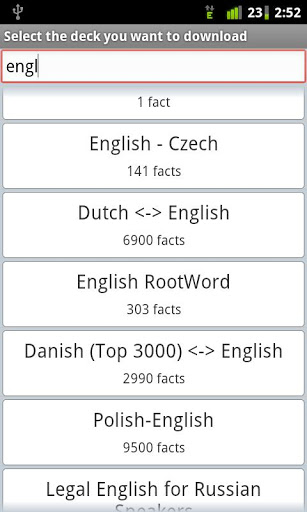
\includegraphics[width=5cm]{Screenshot3}
\caption{AnkiDroid Screenshot : Loading existing deck from a web service.}
\end{figure}




\section{Standards overview, short comparison}

%\begin{figure}[t]
%\centering
%\label{fig:Importantpoints}
%\includegraphics[width=14cm]{Focus}
%\caption{Safety Standards}
%\end{figure}

In electrical, electronic and programmable electronic  (E/E/PE) systems development certain standards
exist. Following the standards is necessary, in particular, for the end product to pass the certification
and be allowed for production and usage.

The safety standards are usually application-domain specific.

What we're talking about (see Figure \ref{fig:Importantpoints}).


\section{Development cycle intro, V-Model}


\section{Standard Case : ISO 26262}
\subsection{System Level Development}
\subsection{Development on the Software Level}


\section{Introduction to Safety Integrity Classes}

The core points, concisely explained with a clear content derivation. (See Table \ref{tab:boringdetails}, more details in section \ref{sec:details}).

explains the basics of functional safety.

\begin{table*}[h]
\centering
\label{tab:boringdetails}
\begin{tabular}{|c|c|l|} \hline
C & C & C\\ \hline\hline
text & 100 & text \\ \hline
text & 200 & text \\ \hline
text & 300 & text \\ \hline
text & 400 & text \\ \hline
\end{tabular}
\caption{For tabular representations}
\end{table*}

%\input{additionalfile} 

\section{Conclusion}

Lessons learned or especially noteworthy info.




\bibliography{idea}



\begin{appendix}
\section{Appendix and addendums}
\label{sec:details}

%\input{details}	

Special focus areas or extra info that is not specifically placeable within the above sequences.

\end{appendix}


\end{document}
